% !TeX spellcheck = en_GB
\section{Results}
\label{sec_results}

In the following we present the results from the two scenarios.

\subsection{Dynamic distance}

\begin{figure}		
	
	\begin{tikzpicture}
\begin{axis}
[
width=0.8\textwidth,
xlabel=meter,
ylabel=dBm,
xtick={1, 2, 3, 4, 5, 6, 7, 8, 9, 10, 11, 12, 13, 14},
xticklabels={0.5, 1, 2, 3, 4, 6, 8, 10, 12, 14, 16, 18, 20},
boxplot/draw direction=y
]


%"00.5"                                
\buildBoxPlot{-50}{-46}{-59}{-73}{-43} 
%%"00"                                  
%\buildBoxPlot{-26}{-26}{-27}{-30}{-25} 
%"01"                                  
\buildBoxPlot{-55}{-54}{-58}{-63}{-47} 
%"02"                                  
\buildBoxPlot{-55}{-48}{-58}{-79}{-44} 
%"03"                                  
\buildBoxPlot{-63}{-60}{-66}{-85}{-53} 
%"04"                                  
\buildBoxPlot{-63}{-60}{-68}{-89}{-51} 
%%"05"                                  
%\buildBoxPlot{-68}{-65}{-71}{-84}{-59} 
%"06"                                  
\buildBoxPlot{-69}{-67}{-71}{-90}{-61} 
%%"07"                                  
%\buildBoxPlot{-73}{-68}{-78}{-92}{-63} 
%"08"                                  
%\buildBoxPlot{-73}{-68}{-77}{-90}{-60} 
%%"09"                                  
\buildBoxPlot{-69}{-64}{-71}{-91}{-59} 
%"10"                                  
\buildBoxPlot{-71}{-67}{-75}{-92}{-62} 
%"12"                                  
\buildBoxPlot{-78}{-75}{-82}{-94}{-66} 
%"14"                                  
\buildBoxPlot{-70}{-68}{-73}{-81}{-60} 
%"16"                                  
\buildBoxPlot{-69}{-68}{-77}{-93}{-63} 
%"18"                                  
\buildBoxPlot{-75}{-71}{-78}{-93}{-65} 
%"20"                                  
\buildBoxPlot{-77}{-74}{-80}{-91}{-66} 


\addplot[thick, red] coordinates {
	(1  ,-50)
	(2  ,-55)
	(3  ,-55)
	(4  ,-63)	
	(5  ,-63)	
	(6  ,-69)	
	(7  ,-69)
	(8  ,-71)
	(9  ,-78)
	(10 ,-70)
	(11 ,-69)
	(12 ,-75)
	(13 ,-77)
	
	};
\end{axis}


\end{tikzpicture}
	
	\caption{ Dynamic distance measurements 1 }
	\label{graf_hopper1}
	
\end{figure}

\begin{figure}		
	
	\begin{tikzpicture}
\begin{axis}
[
xlabel=meter,
ylabel=dBm,
xtick={1, 2, 3, 4, 5, 6, 7, 8, 9, 10, 11, 12, 13, 14},
xticklabels={0.5, 1, 2, 3, 4, 6, 8, 10, 12, 14, 16, 18, 20},
boxplot/draw direction=y
]


%%"00"
%\buildBoxPlot{-19}{-18}{-22}{-23}{-18}
%"00.5"
\buildBoxPlot{-43}{-42}{-45}{-49}{-41}
%"01"
\buildBoxPlot{-50}{-48}{-52}{-63}{-44}
%"02"
\buildBoxPlot{-58}{-53}{-62}{-81}{-46}
%"03"
\buildBoxPlot{-61}{-58}{-65}{-86}{-49}
%%"05"
%\buildBoxPlot{-64}{-62}{-66}{-80}{-55}
%"04"
\buildBoxPlot{-63}{-58}{-66}{-85}{-52}
%"06"
%\buildBoxPlot{-62}{-59}{-70}{-78}{-53}
%%"07"
\buildBoxPlot{-65}{-61}{-67}{-83}{-51}
%"08"
%\buildBoxPlot{-70}{-68}{-74}{-89}{-60}
%%"09"
\buildBoxPlot{-73}{-70}{-77}{-92}{-62}
%"12"
\buildBoxPlot{-62}{-61}{-64}{-75}{-57}
%"10"
\buildBoxPlot{-65}{-62}{-70}{-90}{-57}
%"16"
\buildBoxPlot{-63}{-62}{-65}{-71}{-56}
%"20"
\buildBoxPlot{-71}{-71}{-72}{-85}{-67}
%"14"
\buildBoxPlot{-68}{-64}{-71}{-81}{-57}
%"18"
\buildBoxPlot{-75}{-73}{-80}{-91}{-69}


\addplot[thick, red] coordinates {
	(1  ,-43)
	(2  ,-50)
	(3  ,-58)	
	(4  ,-61)	
	(5  ,-63)	
	(6  ,-65)
	(7  ,-73)
	(8  ,-62)
	(9 ,-65)
	(10 ,-63)
	(11 ,-71)
	(12 ,-68)
	(13 ,-75)
		
};

\end{axis}

\end{tikzpicture}
	
	\caption{ Dynamic distance measurements 2 }
	\label{graf_hopper2}
	
\end{figure}

\begin{figure}		
	
	\begin{tikzpicture}
\begin{axis}
[
xlabel=meter,
ylabel=dBm,
xtick={1, 2, 3, 4, 5, 6, 7, 8, 9, 10, 11, 12, 13, 14},
xticklabels={0.5, 1, 2, 3, 4, 6, 8, 10, 12, 14, 16, 18, 20},
boxplot/draw direction=y
]


%%"00"                                   
%\buildBoxPlot{-36}{-31}{-39}{-43}{-30}  
%"00.5"                                 
\buildBoxPlot{-55}{-50}{-61}{-83}{-46}  
%"01"                                   
\buildBoxPlot{-49}{-47}{-62}{-81}{-41}  
%"02"                                   
\buildBoxPlot{-55}{-51}{-59}{-77}{-46}  
%"03"                                   
\buildBoxPlot{-66}{-60}{-71}{-76}{-57}  
%"04"                                   
\buildBoxPlot{-60}{-55}{-62}{-65}{-52}  
%%"05"                                   
%\buildBoxPlot{-65}{-63}{-68}{-88}{-58}  
%"06"                                   
\buildBoxPlot{-66}{-65}{-68}{-78}{-59}  
%%"07"                                   
%\buildBoxPlot{-69}{-66}{-74}{-83}{-62}  
%"08"                                   
\buildBoxPlot{-63}{-62}{-75}{-83}{-59}  
%%"09"                                   
%\buildBoxPlot{-65}{-61}{-67}{-69}{-57}  
%"10"                                   
\buildBoxPlot{-63}{-62}{-65}{-72}{-57}  
%"12"                                   
\buildBoxPlot{-66}{-64}{-68}{-78}{-59}  
%"14"                                   
\buildBoxPlot{-67}{-66}{-69}{-91}{-63}  
%"16"                                   
\buildBoxPlot{-69}{-67}{-71}{-87}{-59}  
%"18"                                   
\buildBoxPlot{-73}{-71}{-76}{-88}{-65}  
%"20"                                   
\buildBoxPlot{-75}{-72}{-77}{-91}{-67}  


\addplot[thick, red] coordinates {
	(1  ,-55)
	(2  ,-49)
	(3  ,-55)	
	(4  ,-66)	
	(5  ,-60)	
	(6  ,-66)
	(7  ,-63)
	(8  ,-63)
	(9 ,-66)
	(10 ,-67)
	(11 ,-69)
	(12 ,-73)
	(13 ,-75)
	
};

\end{axis}

\end{tikzpicture}
	
	\caption{ Dynamic distance measurements 3 }
	\label{graf_hopper3}
	
\end{figure}

\begin{figure}		
	
	\begin{tikzpicture}
\begin{axis}
[
xlabel=meter,
ylabel=dBm,
xtick={1, 2, 3, 4, 5, 6, 7, 8, 9, 10, 11, 12, 13, 14},
xticklabels={0.5, 1, 2, 3, 4, 6, 8, 10, 12, 14, 16, 18, 20},
boxplot/draw direction=y
]


%%"00"                                 
%\buildBoxPlot{-13}{-12}{-15}{-16}{-10}
%"00.5"                               
\buildBoxPlot{-46}{-44}{-47}{-51}{-41}
%"01"                                 
\buildBoxPlot{-62}{-60}{-70}{-91}{-52}
%"02"                                 
\buildBoxPlot{-61}{-60}{-62}{-71}{-53}
%"03"                                 
\buildBoxPlot{-67}{-61}{-71}{-77}{-55}
%"04"                                 
\buildBoxPlot{-65}{-64}{-67}{-84}{-60}
%%"05"                                 
%\buildBoxPlot{-72}{-69}{-75}{-93}{-65}
%"06"                                 
\buildBoxPlot{-68}{-64}{-71}{-76}{-62}
%%"07"                                 
%\buildBoxPlot{-71}{-69}{-75}{-80}{-65}
%"08"                                 
\buildBoxPlot{-71}{-68}{-74}{-84}{-65}
%%"09"                                 
%\buildBoxPlot{-71}{-68}{-79}{-91}{-65}
%"10"                                 
\buildBoxPlot{-71}{-71}{-72}{-77}{-67}
%"12"                                 
\buildBoxPlot{-70}{-67}{-73}{-75}{-64}
%"14"                                 
\buildBoxPlot{-77}{-75}{-80}{-94}{-63}
%"16"                                 
\buildBoxPlot{-71}{-70}{-75}{-84}{-68}
%"18"                                 
\buildBoxPlot{-78}{-75}{-86}{-92}{-69}
%"20"                                 
\buildBoxPlot{-82}{-79}{-83}{-93}{-72} 


\addplot[thick, red] coordinates {
	(1  ,-46)
	(2  ,-62)
	(3  ,-61)	
	(4  ,-67)	
	(5  ,-65)	
	(6  ,-68)
	(7  ,-71)
	(8  ,-71)
	(9 ,-70)
	(10 ,-77)
	(11 ,-71)
	(12 ,-78)
	(13 ,-82)
	
};

\end{axis}

\end{tikzpicture}
	
	\caption{ Dynamic distance measurements 4 }
	\label{graf_hopper4}
	
\end{figure}

%\begin{figure}		
%	
%	\begin{tikzpicture}
  \begin{axis}
    [
	xlabel=meter,
	ylabel=dBm,
	xtick={1, 2, 3, 4, 5, 6, 7, 8, 9, 10, 11, 12},
    xticklabels={0, 2, 4, 6, 8, 10, 12, 14, 16, 18, 20},
    boxplot/draw direction=y
    ]
    

%"00,0"
\buildBoxPlot{-46}{ -45}{ -59}{ -63}{ -44}
%"00,5"
%\buildBoxPlot{-55}{ -55}{ -58}{ -60}{ -54}
%"01"
%\buildBoxPlot{-68}{ -67}{ -69}{ -72}{ -65}
%"02"
\buildBoxPlot{-70}{ -68}{ -74}{ -78}{ -65}
%"04"
\buildBoxPlot{-69}{ -69}{ -71}{ -72}{ -67}
%"06"
\buildBoxPlot{-78}{ -77}{ -78}{ -79}{ -73}
%"08"
\buildBoxPlot{-78}{ -77}{ -83}{ -83}{ -76}
%"10"
\buildBoxPlot{-78}{ -77}{ -79}{ -81}{ -75}
%"12"
\buildBoxPlot{-80}{ -78}{ -81}{ -84}{ -76}
%"14"
\buildBoxPlot{-77}{ -76}{ -77}{ -78}{ -75}
%"18"
\buildBoxPlot{-85}{ -83}{ -85}{ -89}{ -81}
%"16"
\buildBoxPlot{-81}{ -80}{ -81}{ -83}{ -78}
%"20"
\buildBoxPlot{-84}{ -83}{ -84}{ -87}{ -82}


\end{axis}
	
\end{tikzpicture}

%	
%	\caption{ Dynamic distance measurements Filtered }
%	\label{graf_DynamicMesurementsFiltered}
%	
%\end{figure}

The data from this scenario is presented in \cref{graf_hopper1} to \cref{graf_hopper4}.
The figure shows RSSI value at 2 meter intervals between the base station and the mobile phone.
If we look at the median of the measurements there seems to be an exponential decreasing relation between distance and RSSI value.
We also see that measurements on the low side of the mean values has a wider distribution than on the high side of the mean measurements.

\subsection{Static distance}
\begin{figure}
	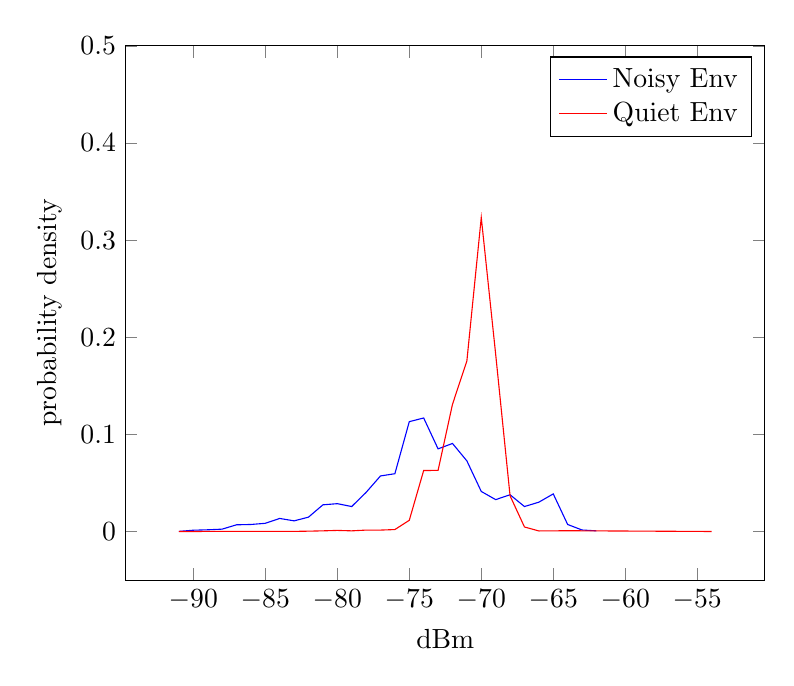
\begin{tikzpicture}
\begin{axis}[
width=0.8\textwidth,
ymax=0.5,
xlabel=dBm,
ylabel=probability density]
\addplot[blue!20!blue] coordinates {
	(-91 ,0.0001093255)
	(-90 ,0.0013119055)
	(-89 ,0.0017492074)
	(-88 ,0.0024051602)
	(-87 ,0.0068875041)
	(-86 ,0.0072154805)
	(-85 ,0.0084180606)
	(-84 ,0.0134470318)
	(-83 ,0.0109325462)
	(-82 ,0.0147589374)
	(-81 ,0.0274406909)
	(-80 ,0.028643271)
	(-79 ,0.0256914835)
	(-78 ,0.04023177)
	(-77 ,0.0571772166)
	(-76 ,0.0594730513)
	(-75 ,0.1130425276)
	(-74 ,0.1168689188)
	(-73 ,0.0850552094)
	(-72 ,0.0906308079)
	(-71 ,0.0727014322)
	(-70 ,0.0412156991)
	(-69 ,0.0327976386)
	(-68 ,0.0378266098)
	(-67 ,0.0256914835)
	(-66 ,0.0301738275)
	(-65 ,0.0387012135)
	(-64 ,0.0072154805)
	(-63 ,0.0015305565)
	(-62 ,0.0006559528)

		};
\addplot[red!20!red] coordinates {
	(-91, 0)
	(-87, 0.0001107297)
	(-86, 0.0001107297)
	(-83, 0.0001107297)
	(-82, 0.0003321891)
	(-81, 0.0006643783)
	(-80, 0.0011072971)
	(-79, 0.0006643783)
	(-78, 0.0014394862)
	(-77, 0.0014394862)
	(-76, 0.0019931348)
	(-75, 0.0115158897)
	(-74, 0.0627837449)
	(-73, 0.0628944746)
	(-72, 0.1308825158)
	(-71, 0.1755065884)
	(-70, 0.3232200199)
	(-69, 0.1824825601)
	(-68, 0.0367622633)
	(-67, 0.0046506478)
	(-66, 0.0005536485)
	(-64, 0.000775108)
	(-54, 0)
	};
\legend{Noisy Env,Quiet Env}
\end{axis}
\end{tikzpicture}

	
	\caption{Static distance measurements}
	\label{graf_StaticMesurements}
\end{figure}

The data from this scenario is presented in \cref{graf_StaticMesurements}.
The figure shows how measurements are distributed over a period of 20 minutes when the distance between the base station and the mobile phone is static.
The experiment was performed in a quiet and a noisy environment.
As one would expect the RSSI values has a much higher spread in the noisy environment than in the quiet environment. 
 

\section{Discussion}
Seeing how the value of the RSSI measured from the device fluctuates in \cref{graf_hopper1} to \cref{graf_hopper4} it is clear that RSSI is hard to use for distance measurements.
From a mean around 45 when measured right on top of the system the RSSI value drops drastically within the first few meters.
As the device moves further away from the system the RSSI value becomes lower but there is no apparent model to the decline.

The noise seams to fluctuate more towards the noise side of the mean. This suggests that if a lower value is measured it is more reliable then a high value, witch fits in well for authentication purposes.
Since most outliers are in the lower dBm end, there is a greater chance that you will be incorrectly logged out as a result of noise than incorrectly logged in.

Looking at \cref{graf_StaticMesurements} we clearly see that the RSSI value becomes less reliable the more noise there is in the environment.
The Noise level will affect how the hysteresis thresholds should be configured.
With too much noise in the environment the mean value of the graph will become indistinct from the rest.

